\chapter{强化学习}
马尔可夫性质:当一个随机过程在给定现在状态及所有过去状态情况下,其未来状态的条件概率分布仅依赖于当前状态;
换句话说,在给定现在状态时,它与过去状态(即该过程的历史路径)是条件独立的,那么此随机过程即具有马尔可夫性质。

\section{强化学习里的对比思考}
\subsection{策略迭代与值迭代}
先参考\href{https://zhuanlan.zhihu.com/p/55217561}{\texttt{这个回答}}。
策略迭代(Policy iteration)的伪代码如图\ref{fig: policy-iteration}所示。
\begin{figure}[htbp]
	\figskip 
	\centering
	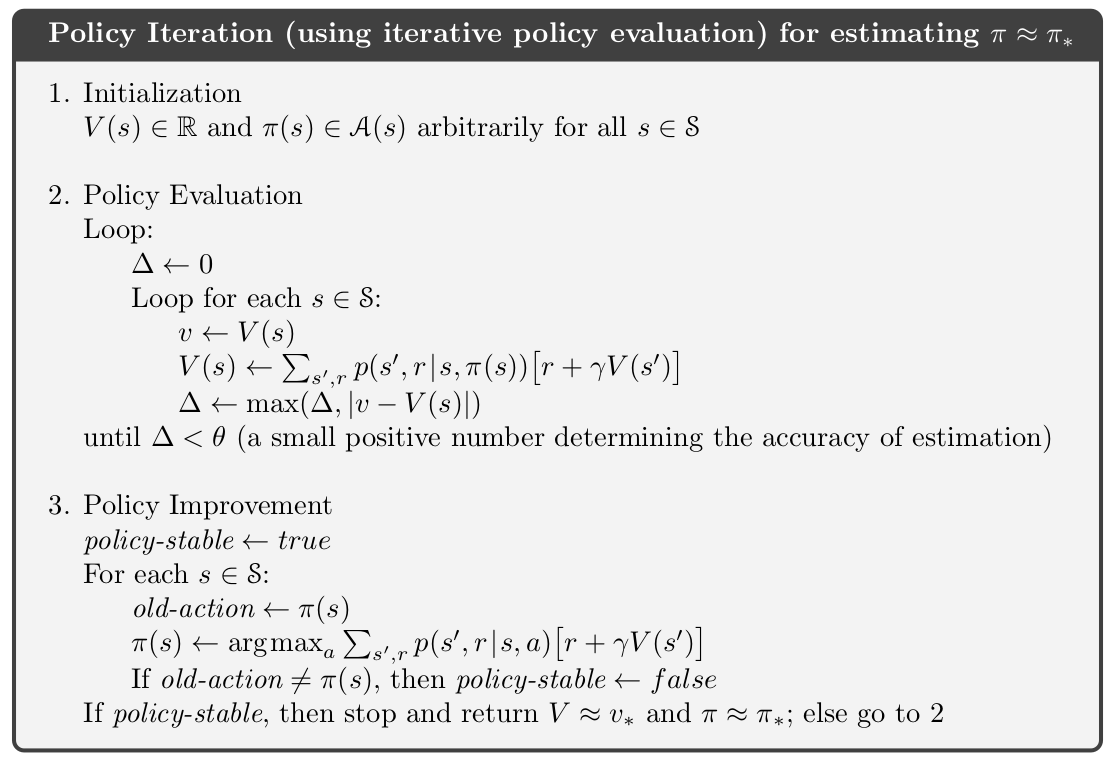
\includegraphics[width = 0.85\textwidth,trim = 0 -0 0 -0,clip]{policy-iteration.png}	  
	\caption{\label{fig: policy-iteration} 策略迭代算法}
\end{figure}
策略迭代中,首先以一个固定的策略(具有概率分布),开始对值函数进行迭代,当值函数稳定后,进行策略提升(更新策略,比如按照greedy的形式)。
然后重复上述步骤直到策略稳定。值迭代(Value iteration)的伪代码如图\ref{fig: value-iteration}所示。
\begin{figure}[htbp]
	\figskip 
	\centering
	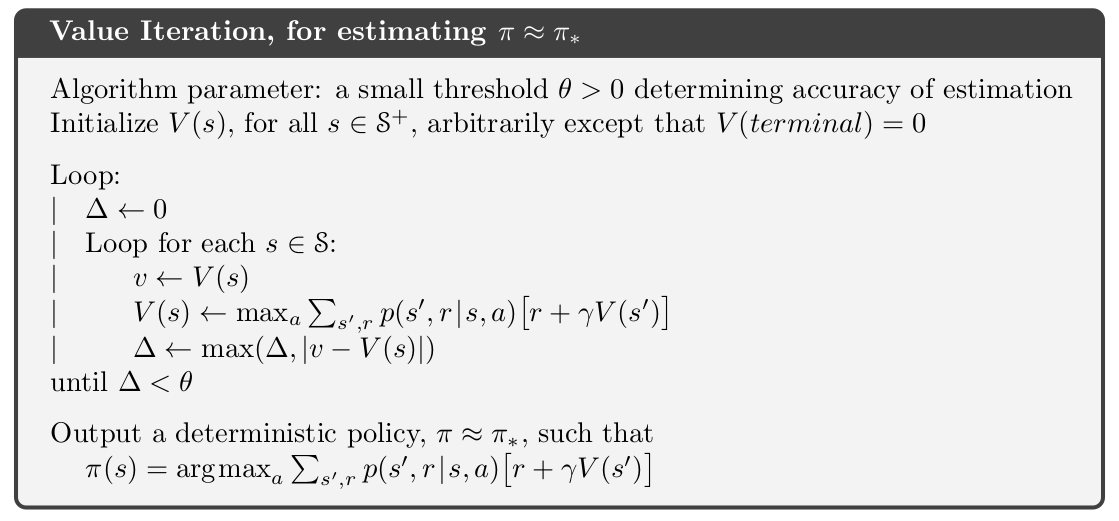
\includegraphics[width = 0.85\textwidth,trim = 0 -0 0 -0,clip]{value-iteration.png}	  
	\caption{\label{fig: value-iteration} 值迭代算法}
\end{figure}
值迭代可以认为策略只选择greedy策略,每做一次值函数迭代,都进行了策略提升(表现在值函数更新时使用的max函数)。


\section{深度强化学习准备知识}
于Model-Free RL,可以分为Policy Optimization和Q-Learning两类方法。
Policy Optimization优化方法包括:PolicyGradient、A2C/A3C、TRPO、PPO等。
Q-Learning方法包括:DQN、C51、QR-DQN、HER等。
此外还有将两种方法融合使用的,包括DDPG、TD3、SAC等。

\begin{figure}[htbp]
	\figskip 
	\centering
	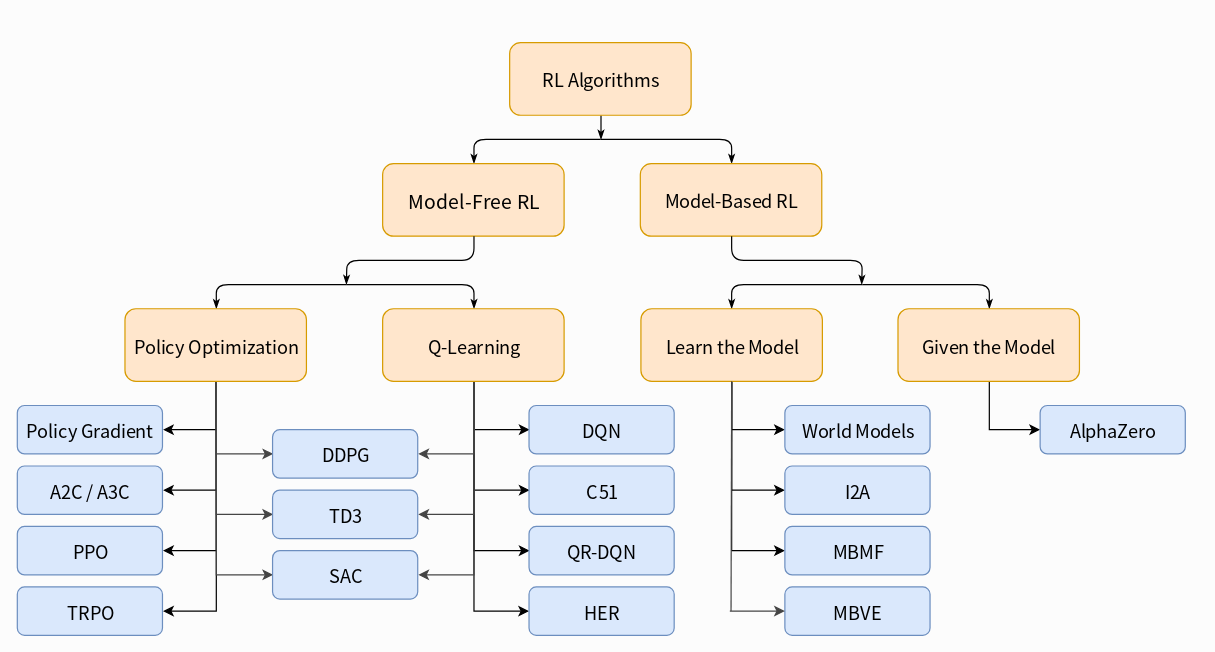
\includegraphics[width = 0.85\textwidth,trim = 0 -0 0 -0,clip]{rl-algorithms.png}	  
	\caption{\label{fig: rl} RL算法的大致分类}
\end{figure}

Policy Optimization 基本思想是直接对策略$\pi_\theta(a|s)$进行估计,
并利用目标函数$J(\pi_\theta)$最优化参数$\theta$。所以这种优化方法绝大部分都是on-policy的方式。
此外在策略优化方法的实现过程中,通常也会采用Actor-Critic的框架。
只不过一般在Policy Optimization中的Critic部分,只进行$V_\phi(s)$的估计。

Q-Learing 基本思想是用$Q_\theta(s,a)$对最优动作值函数进行估计。
通常表现为off-policy的方式。最终的策略可以表示为:
\begin{equation*}
a(s) = \arg \max_a Q_\theta(s,a)
\end{equation*}

而将两种方法结合起来的算法,就是同时估计$Q_\theta(s,a)$和$\pi_\theta(a|s)$

\subsection{Q-Learning 和 Policy Gradient的对比}
参考\href{https://www.zhihu.com/question/49787932}{\texttt{这个问题}}




\subsection{策略分类}
on-policy, off-policy

Deterministic Policies, Stochastic Policies

Categorical Policies, Diagonal Gaussian Policies

\section{DQN}
Q-learning在每步迭代过程中,使用如下的损失函数:
\begin{equation*}
    L_i(\theta_i) = \mathbb{E}_{(s,a,r,s')\sim U(D)} \left[ \left( r+\gamma \max_{a'} \hat{Q}(s',a';\theta_i^-) - Q(s,a;\theta_i) \right)^2 \right]
\end{equation*}

DQN算法的几个核心特点包括:
\begin{enumerate}
    \item 使用CNN完成end-to-end的特征提取及对Q函数的估计
    \item 采用experience replay技巧,削弱episode样本间的相关性,提高算法的收敛的稳定性
    \item 降低target网络的更新频次,增加稳定性
\end{enumerate}

具体算法伪代码为:
\begin{figure}[htbp]
	\figskip 
	\centering
	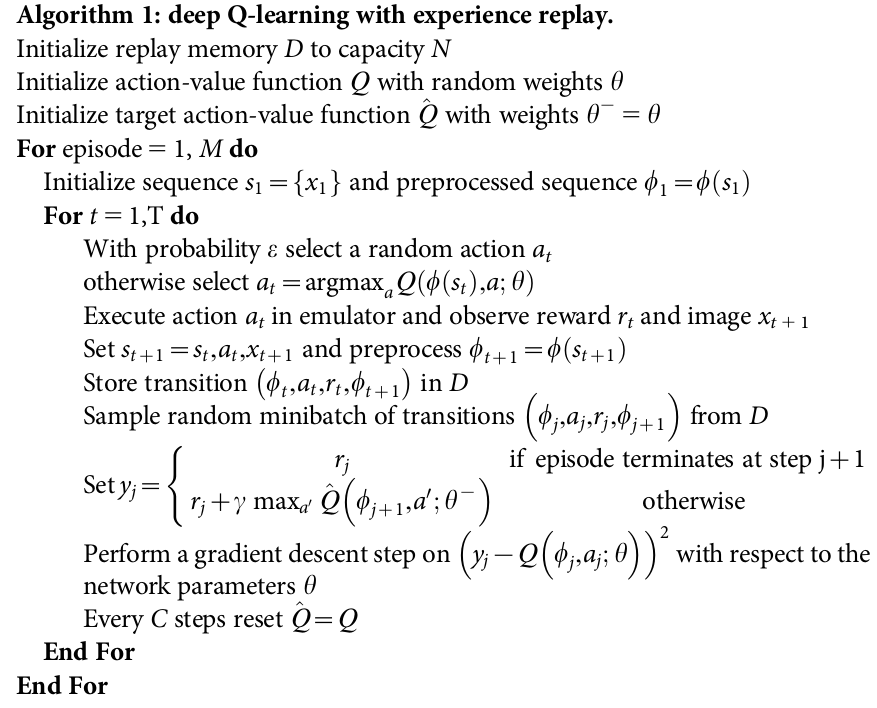
\includegraphics[width = 0.85\textwidth,trim = 0 -0 0 -0,clip]{DQN.png}	  
	\caption{\label{fig: dqn} DQN算法伪代码}
\end{figure}

特点总结:
\begin{enumerate}
    \item off-policy,使用greedy-$\epsilon$的策略做探索,更新greedy策略
    \item 最终保留的是target值函数,即伪代码里的$\hat{Q}(s,a;\theta)$
    \item 离散动作空间,所以$a_{ph}$为1维。
    \item 对于$\max_a Q(s,a;\theta)$的实现,需要对根据s生成的所有$Q(s,\cdot;\theta)$根据$a_{ph}$变量进行切片。使用了tf.gather\_nd()函数
    \item 也可以使用tf.one_hot()进行切片:\texttt{q_sa = tf.reduce_sum(tf.one_hot(a, act_dim) * qvalue, axis=1)}
    \item 两个神经网络间的参数复制,使用tf.assign()函数。
\end{enumerate}

具体代码为
\begin{lstlisting}[language=python,numbers=left,firstnumber = 0,numberstyle=\tiny,breaklines = true,keywordstyle=\color{blue!70},commentstyle=\color{red!50!green!50!blue!50},frame=shadowbox, rulesepcolor=\color{red!20!green!20!blue!20}]
def get_vars(scope):
    return [x for x in tf.global_variables() if scope in x.name]}

self.target_copy = tf.group([tf.assign(v_target, v_value) for v_value, v_target in zip(get_vars('value'), get_vars('target'))])
\end{lstlisting}






\section{策略优化的基础知识}{\label{sec: policy}}
考虑随机性参数化策略$\pi_\theta$,策略的目的是将回报的期望最大化。
因此目标函数为
\begin{equation*}
    J(\pi_\theta) = \mathbb{E}_{\tau\sim\pi_\theta}[R(\tau)]
\end{equation*}

显然可以通过梯度下降的方法对策略进行优化:
\begin{equation*}
    \theta_{k+1} = \theta_k + \alpha \nabla_\theta J(\pi_\theta)|_{\theta_k}
\end{equation*}
其中$\nabla_\theta J(\pi_\theta)$称为策略梯度。
为了使用这个算法,需要显式给出策略梯度的表达式,包括两个步骤:
1)推导出策略性能的分析梯度,结果应该表示成期望的形式。
2)形成该期望值的样本估计,这个估计值可以从有限数量的样本中计算。

对于在策略$\pi_\theta$下采样获得的一条轨迹$\tau = (s_0, a_0, \cdots, s_{T+1})$,其概率为:
\begin{equation*}
    P(\tau|\theta) = \rho_0(s_0) \prod_{t=0}^{T} P(s_{t+1}|s_t, a_t)\pi_\theta(a_t|s_t)
\end{equation*}
考虑对数微分技巧:
\begin{equation*}
    \nabla_\theta P(\tau|\theta) = P(\tau|\theta)\nabla_\theta \log P(\tau|\theta)
\end{equation*}
这样轨迹的对数概率为:
\begin{equation*}
    \log P(\tau|\theta) = \log \rho_0(s_0) + \sum_{t=0}^T \left( \log P(s_{t+1}|s_t,a_t) + \log \pi_\theta (a_t|s_t) \right) 
\end{equation*}
对$\theta$求微分为:
\begin{equation*}
    \nabla_\theta \log P(\tau|\theta) = \sum_{t=0}^T \nabla_\theta \log \pi_\theta(a_t|s_t)
\end{equation*}

计算策略梯度为:
\begin{align*}
    \nabla_\theta J(\pi_\theta) &= \nabla_\theta \mathbb{E}_{\tau\sim\pi_\theta}[R(\tau)] \\
    &= \nabla_\theta \int_\tau P(\tau|\theta)R(\tau) \\
    &= \int_\tau \nabla_\theta P(\tau|\theta)R(\tau) \\
    &= \int_\tau P(\tau|\theta) \nabla_\theta \log P(\tau|\theta)R(\tau) \\
    &= \mathbb{E}_{\tau\sim\pi_\theta}\left[\nabla_\theta \log P(\tau|\theta)R(\tau)\right]
\end{align*}
代入之前的计算结果可得:
\begin{equation}{\label{eq: rl-dj}}
    \nabla_\theta J(\pi_\theta) = \mathbb{E}_{\tau\sim\pi_\theta} \left[ \sum_{t=0}^{T} \nabla_\theta \log \pi_\theta(a_t|s_t) R(\tau) \right]
\end{equation}

式(\ref{eq: rl-dj})是一个期望表达式,那么可以通过采样平均的方式进行估计。
假设我们获得了一个轨迹数据集:$\mathcal{D}=\{\tau_i\}_{i=1,\cdots,N}$,那么策略梯度就可以估计为:
\begin{equation*}
    \hat{g} = \frac{1}{|\mathcal{D}|}\sum_{\tau\in\mathcal{D}}\sum_{t=0}^T \nabla_\theta \log \pi_\theta(a_t|s_t)R(\tau)
\end{equation*}
当使用神经网络优化的方式的时候,通常定义$L(\theta) =\frac{1}{|\mathcal{D}|} \sum_{\tau\in\mathcal{D}}\sum_{t=0}^T \log \pi_\theta(a_t|s_t)R(\tau)$作为损失函数,
这样损失函数的梯度就是策略梯度。

{\hei {几个注意的地方}} 虽然上述定义了一个“损失函数”,但并不意味着它与监督学习里的损失函数具有相同的意义。
具体来说,有一下两点不同:

\noindent {\hei {1. 数据分布依赖于参数。}} 通常损失函数定义在一个固定的数据分布上,与我们待优化的参数是独立的。
但是在这里,数据需要根据最新的策略进行采样。

\noindent {\hei {2. 这里的“损失函数”无法衡量性能。}} 损失函数通常是对我们所关心的性能指标的一种估计。
在这里,我们关系期望回报$J(\pi_\theta)$,但是定义的“损失函数”并不能对其进行估计。这里“损失函数”对我们的作用只是因为,在基于当前待优化参数采样的数据集下,损失函数的梯度与性能梯度相同。
而在完成一次梯度下降之后,二者就没有什么联系了。这意味着,在给定的batch上,最小化损失函数并不能保证一定能够提高期望回报。

\subsection{回报函数}
式(\ref{eq: rl-dj})中在每一个采样状态下都以整条轨迹的回报$R(\tau)$作为当前状态的回报,这显然是不合适的。
通常是否增强当前状态的某个行为,应该考虑执行该行为后的回报,而不是执行之前的历史回报。
所以可以定义如下的"reward-to-go"
\begin{equation*}
    \hat{R}_t \doteq \sum_{t'=t}^T \gamma ^ {t'-t}R(s_{t'}, a_{t'}, s_{t'+1})
\end{equation*}
其中$\gamma$为回报的折扣率。

考虑到可以证明:
\begin{equation*}
    \mathbb{E}_{a_t\sim\pi_\theta}[\nabla_\theta \log \pi_\theta(a_t|s_t)b(s_t)] = 0
\end{equation*}
所以可以在计算策略梯度的时候给回报部分增加一个只与状态相关的值函数$b(s_t)$,称为baseline。
最常规的baseline选择就是当前策略的值函数$V^\pi(s_t)$。那么这个时候相当于用优势函数作为回报。
通常$V^\pi(s-t)$无法直接得到,所以一般也是采用神经网络$V_\phi(s_t)$对最优动作值函数进行估计。

所以一个更为一般形式的策略梯度为:
\begin{equation}{\label{eq: general-pg}}
    \nabla_\theta J(\pi_\theta) = \mathbb{E}_{\tau\sim\pi_\theta} \left[ \sum_{t=0}^T \nabla_\theta \log\pi_\theta(a_t|s_t) \Phi_t \right]
\end{equation}
其中$\Phi_t$可以取为不同形式的函数。

\subsection{Generalized Advantage Estimation, GAE}
假设$V$是Value值函数的一个近似,那么在折扣率$\gamma$下的TD残差可以表示为$\delta_t^V = r_t + \gamma V(s_{t+1}) - V(s_t)$
显然$\delta_t^V$可以看成是优势函数在动作$a_t$下的一个估计。如果值函数是真实的$V = V^{\pi,\gamma}$
\begin{equation*}
    \mathbb{E}_{s_{t+1}}[\delta_t^{V^{\pi,\gamma}}] = \mathbb{E}_{s_{t+1}}[r_t + \gamma V^{\pi,\gamma}(s_{t+1}) - V^{\pi,\gamma}(s_t)] = A^{\pi,\gamma}(s_t, a_t)
\end{equation*}

通过推导可以得到:
\begin{equation*}
    \hat{A}_t^{GAE(\gamma,\lambda)} \doteq \sum_{l=0}^\infty (\gamma \lambda)^l \delta_{t+l}^V
\end{equation*}
表示了一种广义的优势函数的估计。$\lambda$为调节参数:
\begin{gather*}
    \text{GAE}(\gamma,\lambda=0):\, \hat{A}_t = \delta_t = r_t + \gamma V(s_{t+1}) - V(s_t) \\
    \text{GAE}(\gamma,\lambda=1):\, \hat{A}_t = \sum_{l=0}^\infty \gamma^l \delta_{t+1} = \sum_{l=0}^\infty \gamma^l r_{t+1} - V(s_t)
\end{gather*}
$\text{GAE}(\gamma,0)$估计是无偏差的,但会引入较大的方差。$\text{GAE}(\gamma,1)$估计是有偏差的,但是方差较小。

计算GAE的代码:
\begin{lstlisting}[language=python,numbers=left,firstnumber = 0,numberstyle=\tiny,breaklines = true,keywordstyle=\color{blue!70},commentstyle=\color{red!50!green!50!blue!50},frame=shadowbox, rulesepcolor=\color{red!20!green!20!blue!20}]
def discount_cumsum(x, discount):
"""
magic from rllab for computing discounted cumulative sums of vectors.

input: 
    vector x, 
    [x0, 
        x1, 
        x2]

output:
    [x0 + discount * x1 + discount^2 * x2,  
        x1 + discount * x2,
        x2]
"""
return scipy.signal.lfilter([1], [1, float(-discount)], x[::-1], axis=0)[::-1]

deltas = rews[:-1] + self.gamma * vals[1:] - vals[:-1]
self.adv_buf[path_slice] = discount_cumsum(deltas, self.gamma * self.lam)
\end{lstlisting}

\section{DDPG算法}
\subsection{另一种目标函数的形式}
在\ref{sec: policy}节中,定义了目标函数的形式为$ J(\pi_\theta) = \mathbb{E}_{\tau\sim\pi_\theta}[R(\tau)] $。
并推导了在该形式下的策略梯度。
从这个目标函数的定义形式可以看出,其出发点在于考虑每一条轨迹回报,目的是使得在轨迹空间期望回报最大。

在DPG算法之前,首先换一个角度。考虑状态-动作空间中的每一个(s,a)的价值函数$Q(s,a)$,
如果目的是使得状态-动作空间中的价值函数期望最大,那么就可以定义如下形式的目标函数:
\begin{align}{\label{eq: J2}}
    J(\pi_\theta) &= \mathbb{E}_{s\sim\rho^\pi,a\sim\pi_\theta}[Q(s,a)] \notag \\ 
    &= \int_{\mathcal{S}}\rho^\pi(s)\int_{\mathcal{A}}\pi_\theta(s,a)Q(s,a)\dd a \dd s
\end{align}
其中,$\rho^\pi(s)$表示在状态s在一条轨迹中被访问的概率。具体定义为:
\begin{equation*}
    \rho^{\pi}(s') \doteq \int_{\mathcal{S}} \sum_{t=1}^{\infty} \gamma^{t-1} p_0(s) p(s \rightarrow s', t, \pi) \dd s
\end{equation*}
上式右端第三项表示:在策略$\pi$作用下,从状态$s$经过t步转移后到达$s'$的概率。

对式(\ref{eq: J2})求梯度有:
\begin{align*}{}
    \nabla_\theta J(\pi_\theta) &= \nabla_\theta \int_{\mathcal{S}}\rho^\pi(s)\int_{\mathcal{A}}\pi_\theta(s,a)Q(s,a)\dd a \dd s \\
    &= \int_{\mathcal{S}}\rho^\pi(s) \int_{\mathcal{A}} \nabla_\theta \pi_\theta(s,a)Q(s,a)\dd a \dd s \\
    &= \int_{\mathcal{S}}\rho^\pi(s) \int_{\mathcal{A}} \pi_\theta(s,a) \nabla_\theta \log \pi_\theta(s,a)Q(s,a)\dd a \dd s \\
    &= \mathbb{E}_{s\sim\rho^\pi,a\sim\pi_\theta}[\nabla_\theta \log \pi_\theta(s,a)Q(s,a)]
\end{align*}
显然与式(\ref{eq: rl-dj})是等价。

\subsection{确定性策略梯度 DPG}
进一步考虑确定性策略,定义为:
\begin{equation*}
    a = \mu_\theta(s)
\end{equation*}
即在任意状态$s$下都能得到惟一性的动作$a$。代入上一节的目标函数中有:
\begin{align}{\label{eq: J2}}
    J(\theta) &= \mathbb{E}_{s\sim\rho^\mu}[Q(s,\mu_\theta(s))] \notag \\ 
    &= \int_{\mathcal{S}}\rho^\mu(s)Q(s,\mu_\theta(s))\dd s
\end{align}
则策略梯度为:
\begin{align*}
\nabla_\theta J(\theta) &= \int_{\mathcal{S}} \rho^\mu(s) \nabla_\theta \mu_\theta(s) \nabla_a Q^\mu(s,a)|_{a=\mu_\theta(s)} ds \\
&= \mathbb{E}_{s\sim\rho^\mu}\left[ \nabla_\theta \mu_\theta(s) \nabla_a Q^\mu(s,a)|_{a=\mu_\theta(s)} \right]
\end{align*}







